% Thesis template, taken from CVPR 2022 paper template.
% CVPR 2022 Paper Template
% based on the CVPR template provided by Ming-Ming Cheng (https://github.com/MCG-NKU/CVPR_Template)
% modified and extended by Stefan Roth (stefan.roth@NOSPAMtu-darmstadt.de)

\documentclass[10pt,twocolumn,letterpaper]{article}

%%%%%%%%% PAPER TYPE  - PLEASE UPDATE FOR FINAL VERSION
%\usepackage[review]{sarmata}      % To produce the REVIEW version
\usepackage{sarmata}              % To produce the CAMERA-READY version
%\usepackage[pagenumbers]{cvpr} % To force page numbers, e.g. for an arXiv version

% Include other packages here, before hyperref.

\usepackage{multirow}
\usepackage{graphicx}
\usepackage{amsmath}
\usepackage{amssymb}
\usepackage{booktabs}
\usepackage[pagebackref,breaklinks,colorlinks]{hyperref}
\usepackage[none]{hyphenat}
% Support for easy cross-referencing
\usepackage[capitalize]{cleveref}
\crefname{section}{Sec.}{Secs.}
\Crefname{section}{Section}{Sections}
\Crefname{table}{Table}{Tables}
\crefname{table}{Tab.}{Tabs.}


\begin{document}

\begin{titlepage}
    \begin{center}
        % Logos
        
\includegraphics[width=0.3\textwidth]{hhu_logo.png} \hfill \\[1cm]

        {\Large\textsc{Heinrich-Heine-Universität D\"usseldorf}}\\[3cm]
        {\Large\textbf{Bachelor Thesis}}\\[1cm]

        {\Huge\textbf{Implementierung und Evaluation der Reinforcement-Learning-Methoden Self-Play und Liga-Training in der MicroRTS-Umgebung}}\\[2cm]

        {\Large\textbf{{Name!!!!!!!!!!!!!!!!!!!!!!!!!!!!!!!!!!!!!!!!!!!!!!!!!!!!!!!!!!!!!!!!!!!!!!!!!!!!!!}}}\\[2cm]

        \vfill
        % Details
        \begin{tabbing}
            \hspace{4cm} \= \hspace{8cm} \= \\ % Tab stops
            Degree: \> B.Sc. Computer Science \\
            Supervisor: \> Professor Dr. Paul Swoboda \\
            Co-Supervisor: \> Dr. Peter Arndt \\
            Faculty: \> Mathematisch-Naturwissenschaftliche Fakultät \\
        \end{tabbing}

        \vfill % Vertical space

        {\large XXXXXXXXXXX}
    \end{center}
\end{titlepage}

%%%%%%%%% ABSTRACT
\begin{abstract}
    % (???) Wir oder ich?
    Diese Arbeit verbessert einen bestehenden Agenten für das Echtzeit-Strategiespiel (RTS) MicroRTS. RTS-Spiele gelten als anspruchsvolle Domäne für Deep Reinforcement Learning (DRL), da Agenten mit großen kombinatorischen Aktionsräumen, simultanen Entscheidungen sowie verzögerten und oftmals spärlichen Belohnungen umgehen müssen. Als Basismethode verwenden wir Proximal Policy Optimization (PPO). Bei vielen DRL -Trainingsarten, wie bei reinem PPO, kommt man an einen Punkt, an dem der Agent nicht effizient ausschließlich mit PPO weiter trainiert werden kann, weil ausreichend starke Gegner, gegen die man trainieren kann fehlen oder, weil die vorhandenen Gegner nicht divers genug sind, um eine robuste Policy zu entwickeln. Eine naheliegende und einfache Gegenmaßnahme ist Self-Play (SP), das jedoch in der Praxis instabil sein kann und zu Überanpassung oder zyklischen Strategien führt, wodurch die Leistung gegen externe Gegner sinken kann.

    League-Training (LT) stabilisiert SP, indem es eine Population aus Agenten unterschiedlicher Trainingsstände und Rollen aufbaut. Der trainierenden Agent wird gezielt gegen vielfältige Gegner antreten. Unter anderem auch gegen Main-Exploiter, die trainiert wurden, Schwachstellen der aktuellen Policy auszunutzen. Wir evaluieren die resultierenden Agenten in Matches gegen verschiedene Gegnertypen und vergleichen LT mit reinem SP sowie unserem Anfangs-Agenten. Der Anfangs-Agent wurde mit einer Mischung aus Behavior Cloning (BC) und PPO Trainiert. Unsere Ergebnisse zeigen, dass LT Robustheit und Generalisierungsfähigkeit des Agenten gegenüber unterschiedlichen Gegnern erhöht.
\end{abstract}


\tableofcontents
\newpage

%%%%%%%%% BODY TEXT´
\section{Introduction}
\label{sec:intro}
Reinforcement Learning (RL) etablierte sich in den vergangenen Jahren als leistungsstarker Ansatz für die Entwicklung von Agenten in komplexen Umgebungen. Spielumgebungen wie RTS-Spiele stellen dabei eine besondere Herausforderung dar, mit großen Aktionsräumen, langfristiger Planung und simultanen Entscheidungen. Allerdings bieten sie klar definierte Zustandsräume, Belohnungsstrukturen und wiederholbare Experimente, was sie zu idealen und herausfordernden Testumgebungen für die Erforschung von RL-Methoden macht.

MicroRTS ist eine vereinfachte Version von RTS-Spielen, die speziell für die Forschung entwickelt wurde \cite{huang2021gym}. Sie ist diskret und reduziert die visuelle und mechanische Komplexität von großen kommerziellen RTS-Spielen, zum Beispiel StarCraft II. Wärenddessen behält sie die Kernschwierigkeiten, wie Ressourcenmanagement, Einheitenproduktion, Kampfmechaniken und taktische Positionierung, bei. MicroRTS eignet sich deshalb für die systematische Untersuchung von Lernverfahren. MicroRTS enthält weiterhin zahlreiche Trainingsherausforderungen, wie hohe kombinatorische Aktionsräume, verzögerte Belohnungen, Multi-Agent-Interaktionen und es erfordert auch robuster Strategien gegen unterschiedliche Gegner. Beispielsweise muss sich der Agent früh entscheiden, ob er gegen den aktuellen Gegner aggresiv oder defensiv spielen will, was sich auf die gesamte Spielstrategie auswirkt und eine langfristige Planung erfordert.

Ein zentrales Problem des RL ist die Generalisierung gegenüber unterschiedlichen Gegnern und Strategien: Agenten lernen oft Strategien, die stark auf den Trainingsgegner oder eine spezifische Spielsituation zugeschnitten sind. Das führt zu Überanpassung und eingeschränkter Robustheit. SP, Fictitious Self-Play (FSP) und LT sind Ansätze, die dieses Problem adressieren. In SP trainiert der Agent, in dem er gegen sich selbst spielt, was zu einem kontinuierlichen Lernprozess führt, der keine zusätzlichen diversen oder starken Gegner erfordert. Allerdings ist oft das Training instabil, weil es zyklisch lernt. Ein Beispiel: Spielt der Agentzustand B gut gegen A, C gut gegen B und A gut gegen C, könnte der Agent in einem Zyklus gefangen sein, in dem er immer nur den Agentenzustand wieder erlernt, der gegen sich selbst gut ist, aber nicht gegen andere Gegner.
Um die Instabilitäten von reinem SP zu adressieren, wird in FSP nicht gegen den aktuellen Agenten sondern gegen ältere Versionen des Agenten gespielt, was ein zyklisches Lernen verhindert und in zwei Spieler Nullsummenspielen gegen das Nash-Gleichgewicht konvergiert. \cite{heinrich2015fsp}. LT erweitert FSP, indem der Agent gegen historische Gegner aus einer Liga trainiert, die aus verschiedenen Agententypen besteht, beispielsweise aus historischen Trainingsständen oder spezialisierten Strategien \cite{vinyals2019alphastar}. Ziel ist es, die Lernumgebung zu stabilisieren, in der Agenten gegen ein breites Spektrum an Strategien antreten und dadurch robuster werden.

Trotz der theoretischen Vorteile ist die praktische Implementierung von LT in komplexen Umgebungen, wie MicroRTS, mit erheblichen Herausforderungen verbunden. Dazu gehören:

\begin{itemize}
    \item die effiziente Verwaltung und Auswahl von Gegnern für das Training des Main-Agenten und für die spezialisierten Agenten, wie Main-Exploiter,
    \item die Stabilisierung des Trainingsprozesses bei nicht-konstanten Gegnerverteilungen,
    \item der Umgang mit großen Aktionsräumen und spärlichen oder verzögerten Belohnungen und
    \item die Bewertung der tatsächlichen Generalisierungsfähigkeit der trainierten Agenten.
\end{itemize}

Darüberhinaus werden wir die für die unterschiedlichen Trainingsparadigmen die Lernkurve, die Strategiediversität und die Robustheit vergleichen und evaluieren.

Der in diesem Projekt eingesetzte Basis-Agent, wird in einem dreistufigen Verfahren trainiert, das BC und BC-Fine-Tuning (BC-FT) mit anschließendem Fine-Tuning durch PPO kombiniert: 
Die beiden BC-Phasen ermöglichen es dem Agenten, durch Imitation von Expertenverhalten schnell eine kompetente Basisstrategie zu erlernen \cite{torabi2018behavioral}. Dieser Ansatz des Trainings reduziert die anfängliche, oft ineffiziente Exploration in DRL \cite{torabi2018behavioral}. Das Lernen von Grund auf mit DRL-Methoden wie PPO kann sehr zeitintensiv sein \cite{martin2021beclone}. PPO ist eine bekannte on-policy Policy-Optimierungsmethode, die die Policy-Update-Größe über eine Clipped-Surrogat-Zielfunktion begrenzt \cite{schulman2017ppo}.
PPO verbessert weiterhin die Leistung des BC-Agenten durch Exploration und Anpassung an die Umgebung, wodurch sich der Agent über die Expertenstrategien hinaus anpassen und generalisieren kann \cite{martin2021beclone}. Dieser zweistufige Ansatz, bei dem eine mit BC vor-trainierte Policy durch einen DRL-Algorithmus verfeinert wird, hat sich als effektiv erwiesen, um die Trainingszeit zu verkürzen und die Gesamtleistung im Vergleich zu einem reinen DRL-Ansatz zu verbessern \cite{martin2021beclone}.





\section{Related Work}
\label{sec:related-work}
\noindent\textbf{Game Playing Agents in MicroRTS}
Die dieser Arbeit zugrunde liegende (unveröffentlichte) Bachelorarbeit von Huft entwickelt einen wettbewerbsfähigen Agenten für MicroRTS und evaluiert eine hybride Trainingspipeline aus BC, BC-Fine-Tuning (BC-FT) und anschließendem PPO-Training \cite{huft2023microrts}. Aufbauend auf der in der Introduction beschriebenen Grundidee wird die initiale Policy aus Demonstrationen von Experten gelernt. In BC-FT wird dies mit selektierten Winning-Replays für die Stabilisierung weitergeführt und erst im dritten Schritt durch PPO weiter verfeinert. Dieses stufenweise Vorgehen reduziert die anfängliche Explorationslast und verbessert die Stabilität gegenüber einem reinen DRL-Start.

In den Ergebnissen ist ein deutlicher Leistungsanstieg über alle drei Trainingsphasen zu sehen (Tabelle~\ref{tab:winrates_all}): BC lernt größtenteils grundlegende Spielmechaniken, während BC-FT Generalisierung gegen mehrere Bots verbessert. 
Schließlich erreicht PPO hohe Winrates gegen viele der Built-in-Bots \cite{huft2023microrts}. 
In den Ergebnissen sind Agenten, gegen die der Basis-Agent nicht gut abschneidet. Die Arbeit identifiziert zudem Einschränkungen, insbesondere den Fokus auf eine einzelne Karte, die begrenzte Gegnerdiversität und schlägt Erweiterungen mit Self-Play- bzw. Liga-Mechanismen vor. 
Genau an diesem Vorschlag setzt diese Arbeit an, indem der bestehende Basis-Agent und der initiale Code um SP und LT erweitert werden.
Die Built-in-Bots von MicroRTS, gegen die unter anderem ausgewertet wird, sind RandomBiasedAI, WorkerRushAI, LightRushA und CoacAI.
\begin{table}[ht]
\centering
\caption{Winrates (\%) for BC, BC-FT, and PPO reported in \cite{huft2023microrts}.}
\label{tab:winrates_all}
\begin{tabular}{lccc}
\hline
\textbf{Bot} & \textbf{BC} & \textbf{BC-FT} & \textbf{PPO} \\
\hline
WorkerRushAI     & 3 & 50 & 99 \\
PassiveAI        & 98& 100& 100 \\
LightRushAI      & 22 & 93 & 99 \\
CoacAI           & 0 & 8 & 96 \\
Mayari           & 0 & 5 & 95 \\
RandomAI         & 52 & 95 & 99\\
RandomBiasedAI   & 18 & 68 & 86\\
rojo             & 0 & 34& 84 \\
mixedBot         & 4 & 44 & 59 \\
izanagi          & 0& 62& 61\\
tiamat           & 11 & 78& 84 \\
droplet          & 0& 31& 59\\
guidedRojoA3N    & 4 & 42& 75 \\
naiveMCTS        & 0 & 5& 3 \\
\hline
\end{tabular}
\end{table}
\vspace{10pt}

\noindent\textbf{MicroRTS-Py (Gym-$\mu$RTS)}
Huang et al. stellen mit \emph{Gym-$\mu$RTS} bzw. \emph{MicroRTS-Py} für unser Environment MicroRTS \cite{Ontanon2013CombinatorialBandit} eine effiziente Gym-kompatible Schnittstelle bereit \cite{huang2021gym}. 
MicroRTS-Py ist eine etablierte und weit verbreitete DRL-Baseline, die die Untersuchung von DRL-Ansätzen in vollständigen Echtzeitstrategiespiel-Szenarien ermöglicht, ohne dass dafür umfangreiche technische Infrastruktur, wie Hochleistungsrechner-Cluster, erforderlich ist \cite{huang2021gym}. 
Desweiteren wurde die \emph{openai/baselines} \cite{baselines} -Implementation von PPO adaptiert, um sie auf MicroRTS-Py anzupassen. 
Einen Großteil dieser Implementation setzen wir in LT ein. Ssie wurde auch zuvor in der PPO Trainingsphasen des Basis-Agenten verwendet \cite{huft2023microrts}.
Zu openai/baselines wurden unter anderem \emph{invalid action masking} und geeignete Aktions-/Beobachtungsrepräsentationen (z.\,B.: GridNet \cite{pmlr-v97-han19a}) sowie architektonische Entscheidungen (wie IMPALA-CNN (eine tiefe Convolutional-Neural-Network-Struktur mit residual blocks zur Verarbeitung gitterbasierter Zustandsrepräsentationen in RL) \cite{espeholt2018impala}) hinzugefügt \cite{huang2021gym}, die abgeändert auch in dem LT-Code noch genutzt werden.
Es wurde in dem Paper überlegt, \emph{Unit Action Simulation} (UAS) statt GridNet zu verwenden. UAS itteriert in jedem Schritt über alle Einheiten und gibt für jede Einheit die möglichen Aktionen zurück, was den Aktionsraum deutlich reduziert.
GridNet hingegen sagt für jede Zelle auf der Karte eine Aktion voraus. Das führt GridNet mit seinem großen Aktionsraum in einem Schritt aus, aber das macht das Training simplistischer \cite{huang2021gym, pmlr-v97-han19a}.
Gegen die Built-in-Bots von MicroRTS, die auf heuristischen Regeln basieren, erreicht die PPO-Implementierung mit invalid action masking und IMPALA-CNN im Durchschnitt eine Winrate von 91\% mit UAS und 84\% mit GridNet.
Letztendlich wurde entschieden, sich auf GridNet zu fokusieren, da die Komplexität geringer ist und die Kompatibilität SP (bzw. LT) erleichtert \cite{huang2021gym}.
SP wurde in der Arbeit auch evaluiert. Allerdings gab es in dem Code ein Bug, der wahrscheinlich die Ergebnisse für SP stark beeinflusst hat \cite{goodfriend2024raisocketai}.
\vspace{10pt}

\noindent\textbf{RAISocketAI}
\cite{goodfriend2024raisocketai} RAISocketAI ist der erste DRL-Agent, der im Jahr 2023 die IEEE MicroRTS Competition gewinnen konnte. 
RaiSocketAI beinhaltet eine Neu-Implementation von MicroRTS-Py, die in unserem Code verwendet wird. 
Unter anderem ist die Datengenerierung über Replays ist eine wichtige Grundlage für BC \cite{huft2023microrts} und es wurde ein Bug in der alten Implementation behoben, der nicht besitzte Recourcen als besitzte Recourcen markierte, wenn der Agent Spieler 2 ist. 
Das führte laut Goodfriend wahrscheinlich dazu, dass SP in der vorherigen Implementation von MicroRTS-Py keine Verbesserungen brachte:
Die RAISocketAI-Implementierung von FSP hat gegen die gleichen Built-in-Bots von MicroRTS wie in MicroRTS-Py eine durchschnittliche Winrate von 91\% erreicht, was deutlich höher ist als 84\% in der vorherigen Implementation. 
Allerdings erreichte FSP gegen CoacAI nur eine 20\% Winrate, wärend die besten vorherigen Implementationen fast immer CoacAI besiegen konnten.
Mit finetuning CoacAI und Mayari wurde die durchschnittliche Winrate gegen die Built-in-Bots auf 98\% erhöht \cite{goodfriend2024raisocketai}.
LT wurde in der Arbeit nicht implementiert oder evaluiert.
\vspace{10pt}

\noindent\textbf{BeClone}
\cite{martin2021beclone} \emph{BeClone} zeigte die Effektivität von BC mit DRL-finetuning in MicroRTS-Py mit einer zweiphasigen Trainingsstrategie für RTS-Agenten: Zuerst wird eine initiale Policy per BC von den Experten gelernt, anschließend erfolgt ein RL-Finetuning mittels \emph{Advantage Actor-Critic} (A2C).
\vspace{10pt}

\noindent\textbf{AlphaStar}
\cite{vinyals2019alphastar} AlphaStar demonstriert, dass LT in komplexen RTS-Domänen entscheidend zur Robustheit beitragen kann. 
Der Agent wurde mit \emph{Imitation Learning} aus menschlichen Replays vortrainiert. Das haben wir in dieser Arbeit mit den BC-Phasen und der PPO-Phase ersetzt. 
Anschließend wird der Agent, wie auch in dieser Arbeit, in einer Liga aus unterschiedlichen Agententypen (Main-Agent, Main-Exploiters, League-Exploiters und historische Snapshots) weitertrainiert, um Überanpassung und Vergessen zu reduzieren und Diversität zu fördern. 
Obwohl MicroRTS und StarCraft II in Komplexität und Repräsentation stark differieren, zeigt sich AlphaStar als ein etabliertes Referenzdesign für die Stabilisierung und Generalisierung von SP, durch ligaartige Matchmaking-Mechanismen und die Einbeziehung von spezialisierten Exploitern \cite{vinyals2019alphastar}.
Wie auch in AlphaStar, werden in dieser Arbeit Main-Exploiters trainiert, indem der Basis-Agent gegen alle historischen Versionen der Main-Agenten in der Liga trainiert wird, um Schwachstellen zu identifizieren und auszunutzen \cite{vinyals2019alphastar}.
Gleichzeitig trainieren League-Exploiters gegen alle \emph{Historischen Agenten} \cite{vinyals2019alphastar}.
Der Main-Agent trainiert mit \emph{prioritized FSP} (PFSP) gegen historische Versionen von sich selbst, Main-Exploiters und League-Exploiters \cite{vinyals2019alphastar}.
Die Priorisierung der historischen Gegneragenten erfolgt durch die Winrate des Main-Agenten gegen die jeweiligen historischen Agenten \cite{vinyals2019alphastar}.
Erst, wenn ein Exploiter eine große Winrate gegenüber allen Gegnern aufweist oder wenn eine bestimmte maximale Schritt-Grenze erreicht ist, wird er in die Liga als Historical (ein historischer Agent) aufgenommen \cite{vinyals2019alphastar}. 
In AlphaStar kommt ein \emph{Actor-Critic-Verfahren} mit einer Off-Policy-Korrekturmethode namens \emph{V-trace} für das Policy-Update zum Einsatz \cite{espeholt2018impala, vinyals2019alphastar}. 
Dieser Ansatz ist durch die Robustheit gegenüber Off-policy-Daten und der typischerweise besseren Skalierbarkeit in großen verteilten Setups besser für LT geeignet als PPO. 
Jedoch ist die Implementierung von PPO in MicroRTS-Py deutlich einfacher und schneller realisierbar, weshalb PPO eine praktikable Wahl für die Umsetzung von LT darstellt \cite{vinyals2019alphastar}.
Dazu wird in AlphaStar \emph{Temporal Difference Learning} (TD($\lambda$)) \cite{suttonbarto1998rl} für die Value-Schätzung verwendet.
% hier weiter arbeiten
\section{Methoden}
\label{sec:Methoden}

% \subsection{Training Pipeline}




\subsection{MicroRTS Environment}
\label{sec:MicroRTS-env}


\begin{itemize}
    \item \(T\) 
    \item \(N\) 
    \item \(H\) 
    \item \(W\) 
    \item \(C\) 
\end{itemize}


\begin{itemize}
    \item 
    \item 
    \item 
    \item 
    \item 
\end{itemize}


\begin{figure}[h]
    \centering
    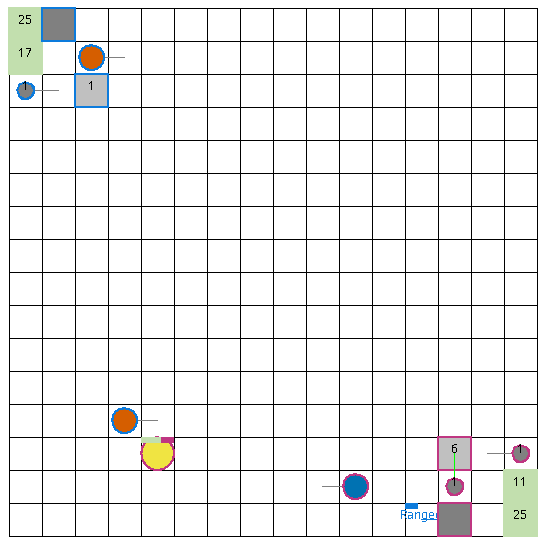
\includegraphics[width=1\linewidth]{images/16x16.png}
    \caption{Screenshot \texttt{basesWorkers16x16A} map. }
    \label{Figure 1}
\end{figure}

% \subsection{Neural Network Architecture}


\label{sec:nn-architecture}

\paragraph{ScalarEncoder}  

\[
\mathrm{ScalarEncoder}:\ \mathbb{R}^{d_{\text{in}}}\rightarrow\mathbb{R}^{d_{\text{out}}},
\]



\begin{figure}[h]
    \centering
    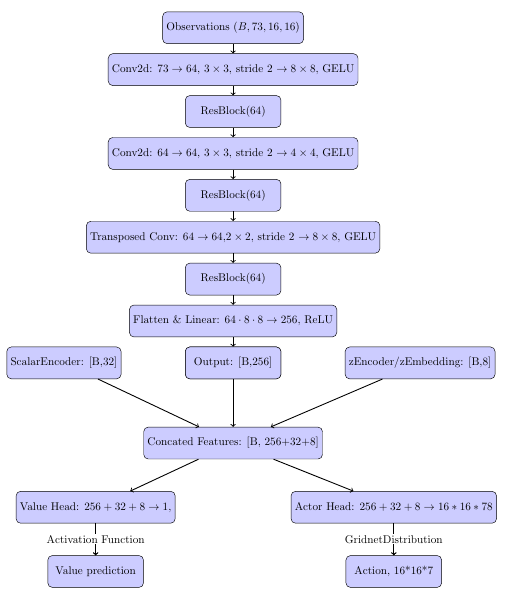
\includegraphics[width=1.1\linewidth, height=10cm]{images/diagram.png}
    \caption{The Network Architecture}
    \label{Figure 2}
\end{figure}




% \subsection{Behavior Cloning}



% \subsection{Reinforcement Training}

\section{Experimente}
\label{sec:experimente}

% \subsection{Setup}
\begin{table}[h]
\centering
\caption{Training parameters for PPO training.}
\begin{tabular}{l c}
\hline
\textbf{Parameter} & \textbf{Value} \\
\hline
Initial learning rate (Adam) & $2.5 \times 10^{-5}$ \\
Rollout steps per environment & 512 \\
Minibatch Size & 3072\\
Max episode length & 2,000 timesteps \\
Discount factor $\gamma$ &  1 \\
Value function coefficient $\beta$ & 0.01 \\
Entropy coefficient $\eta$ & 0.005 \\
Gradient norm threshold $\omega$ &0.5 \\
KL regularization coefficient $\lambda_{\text{KL}}$ & 0.4 \\
GAE parameter $\lambda$ & 0.95 \\
\hline
\end{tabular}
\label{tab:training_params}
\end{table} 

% \subsection{Results}



\begin{figure}[h]
    \centering
    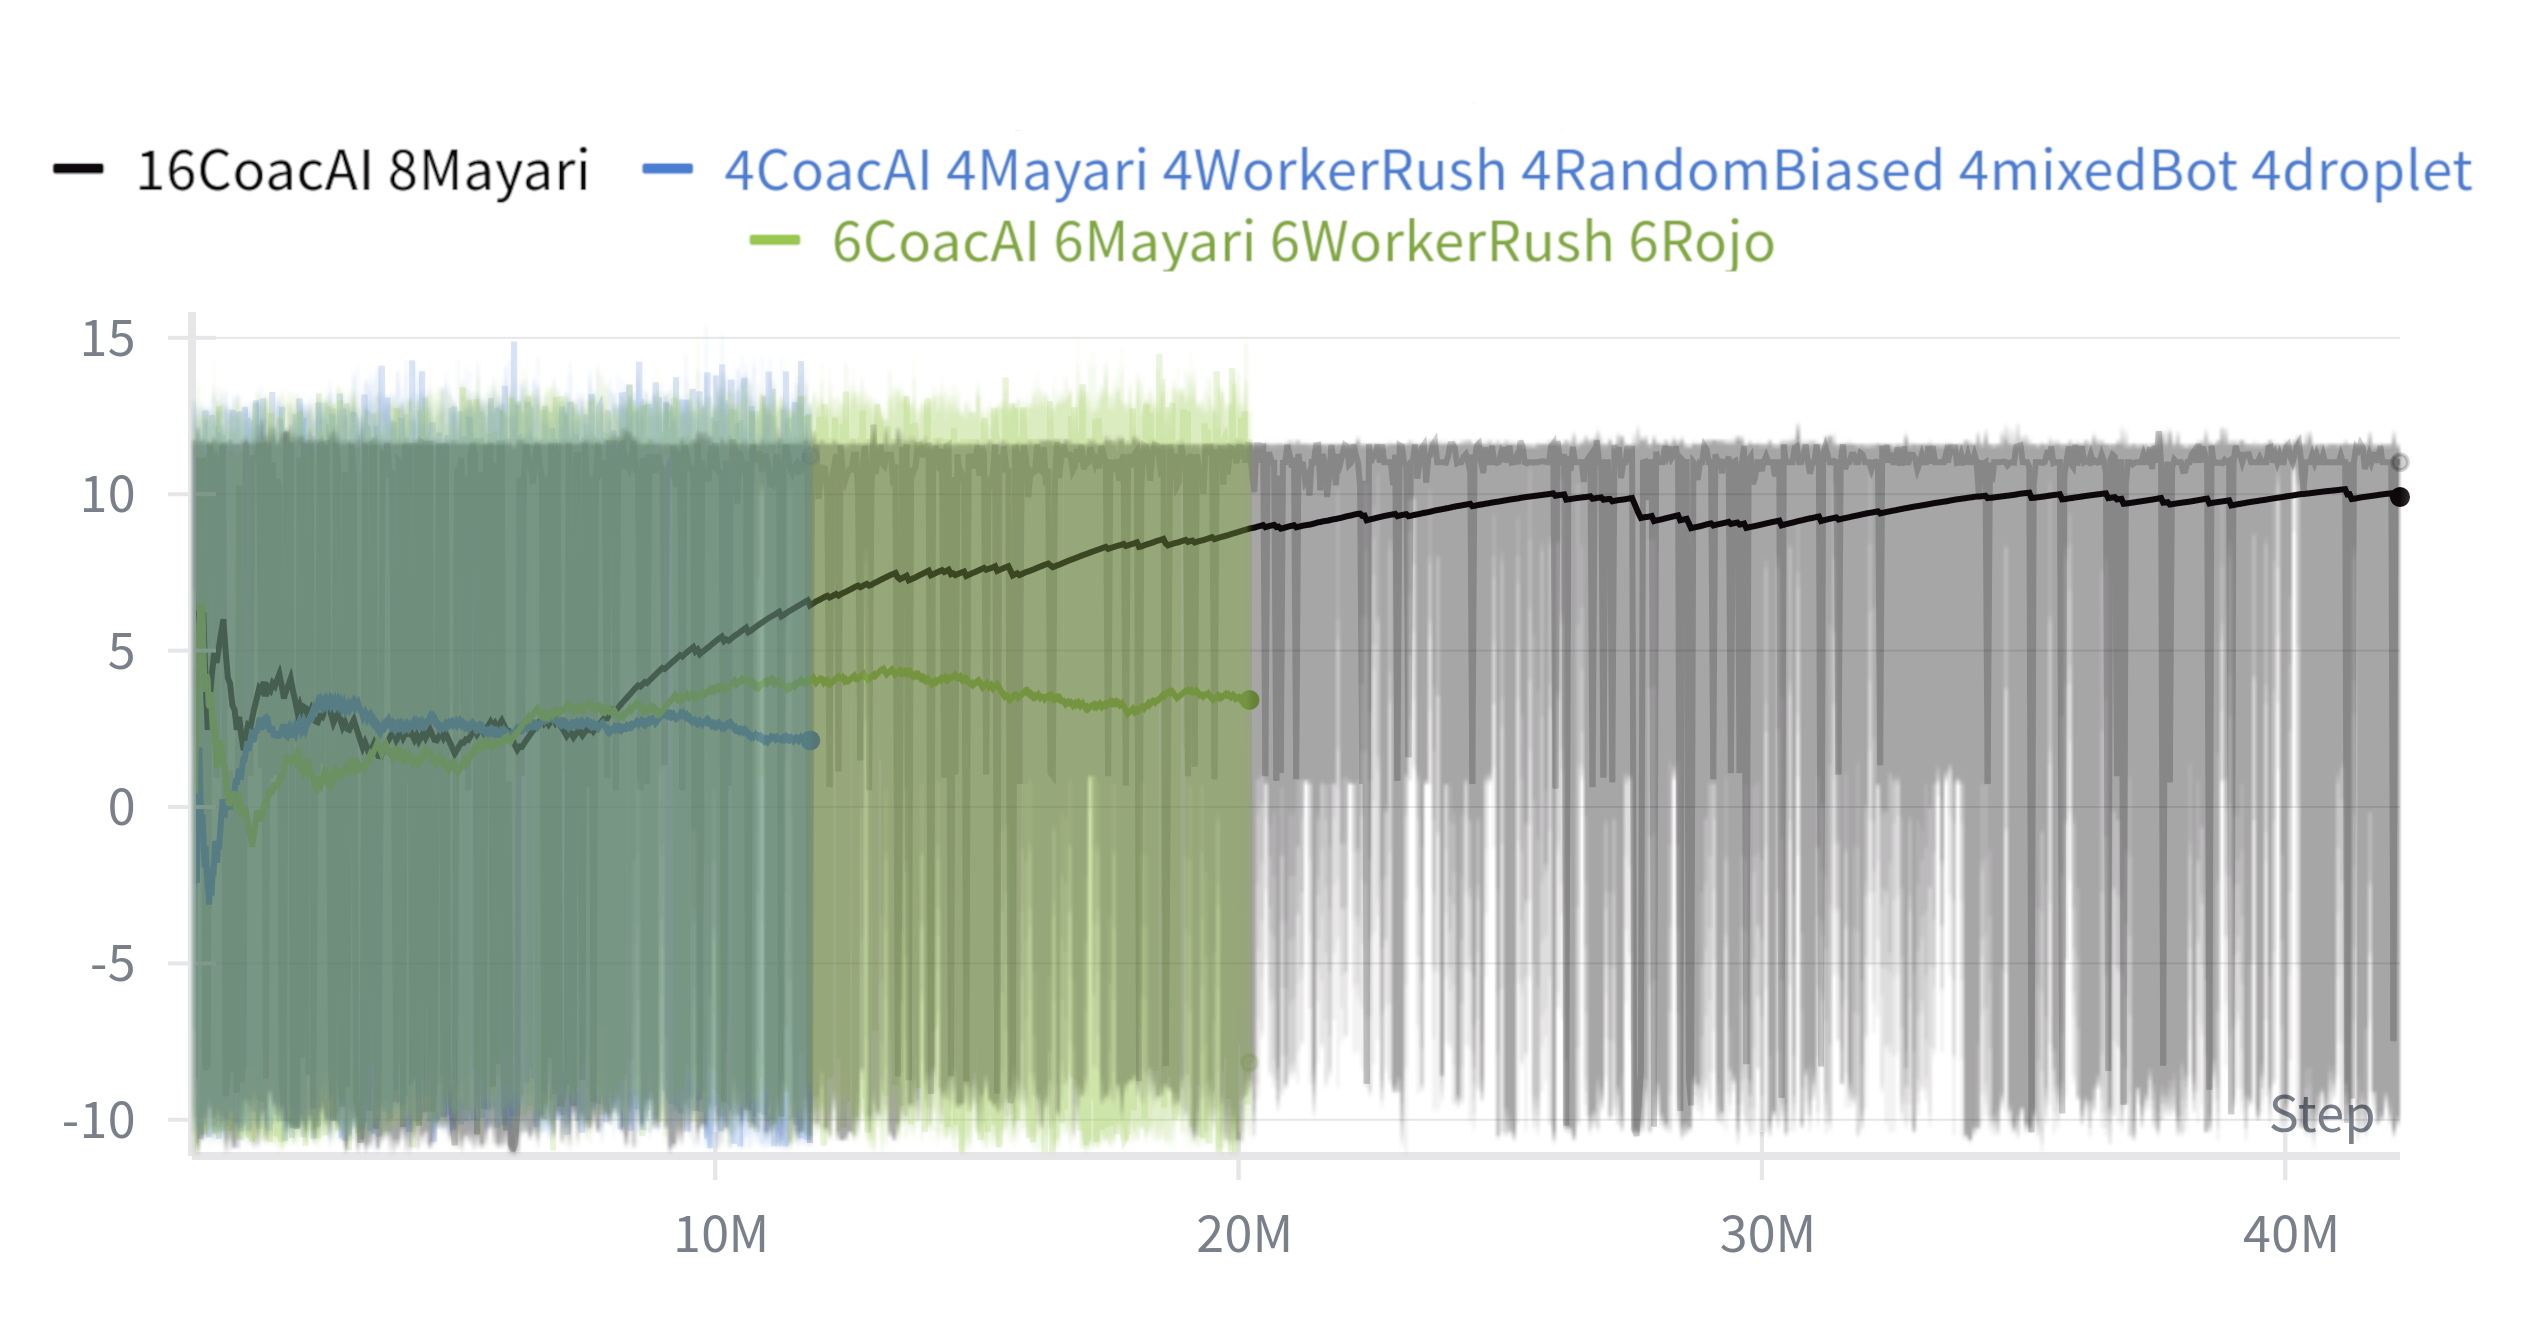
\includegraphics[width=1\linewidth]{images/Fig3.png}
    \caption{Episode rewards (y-axis) as a function of training timesteps (x-axis) on the BC-FT agent.}
    \label{Figure 3}
\end{figure}

\begin{figure}[h]
    \centering
    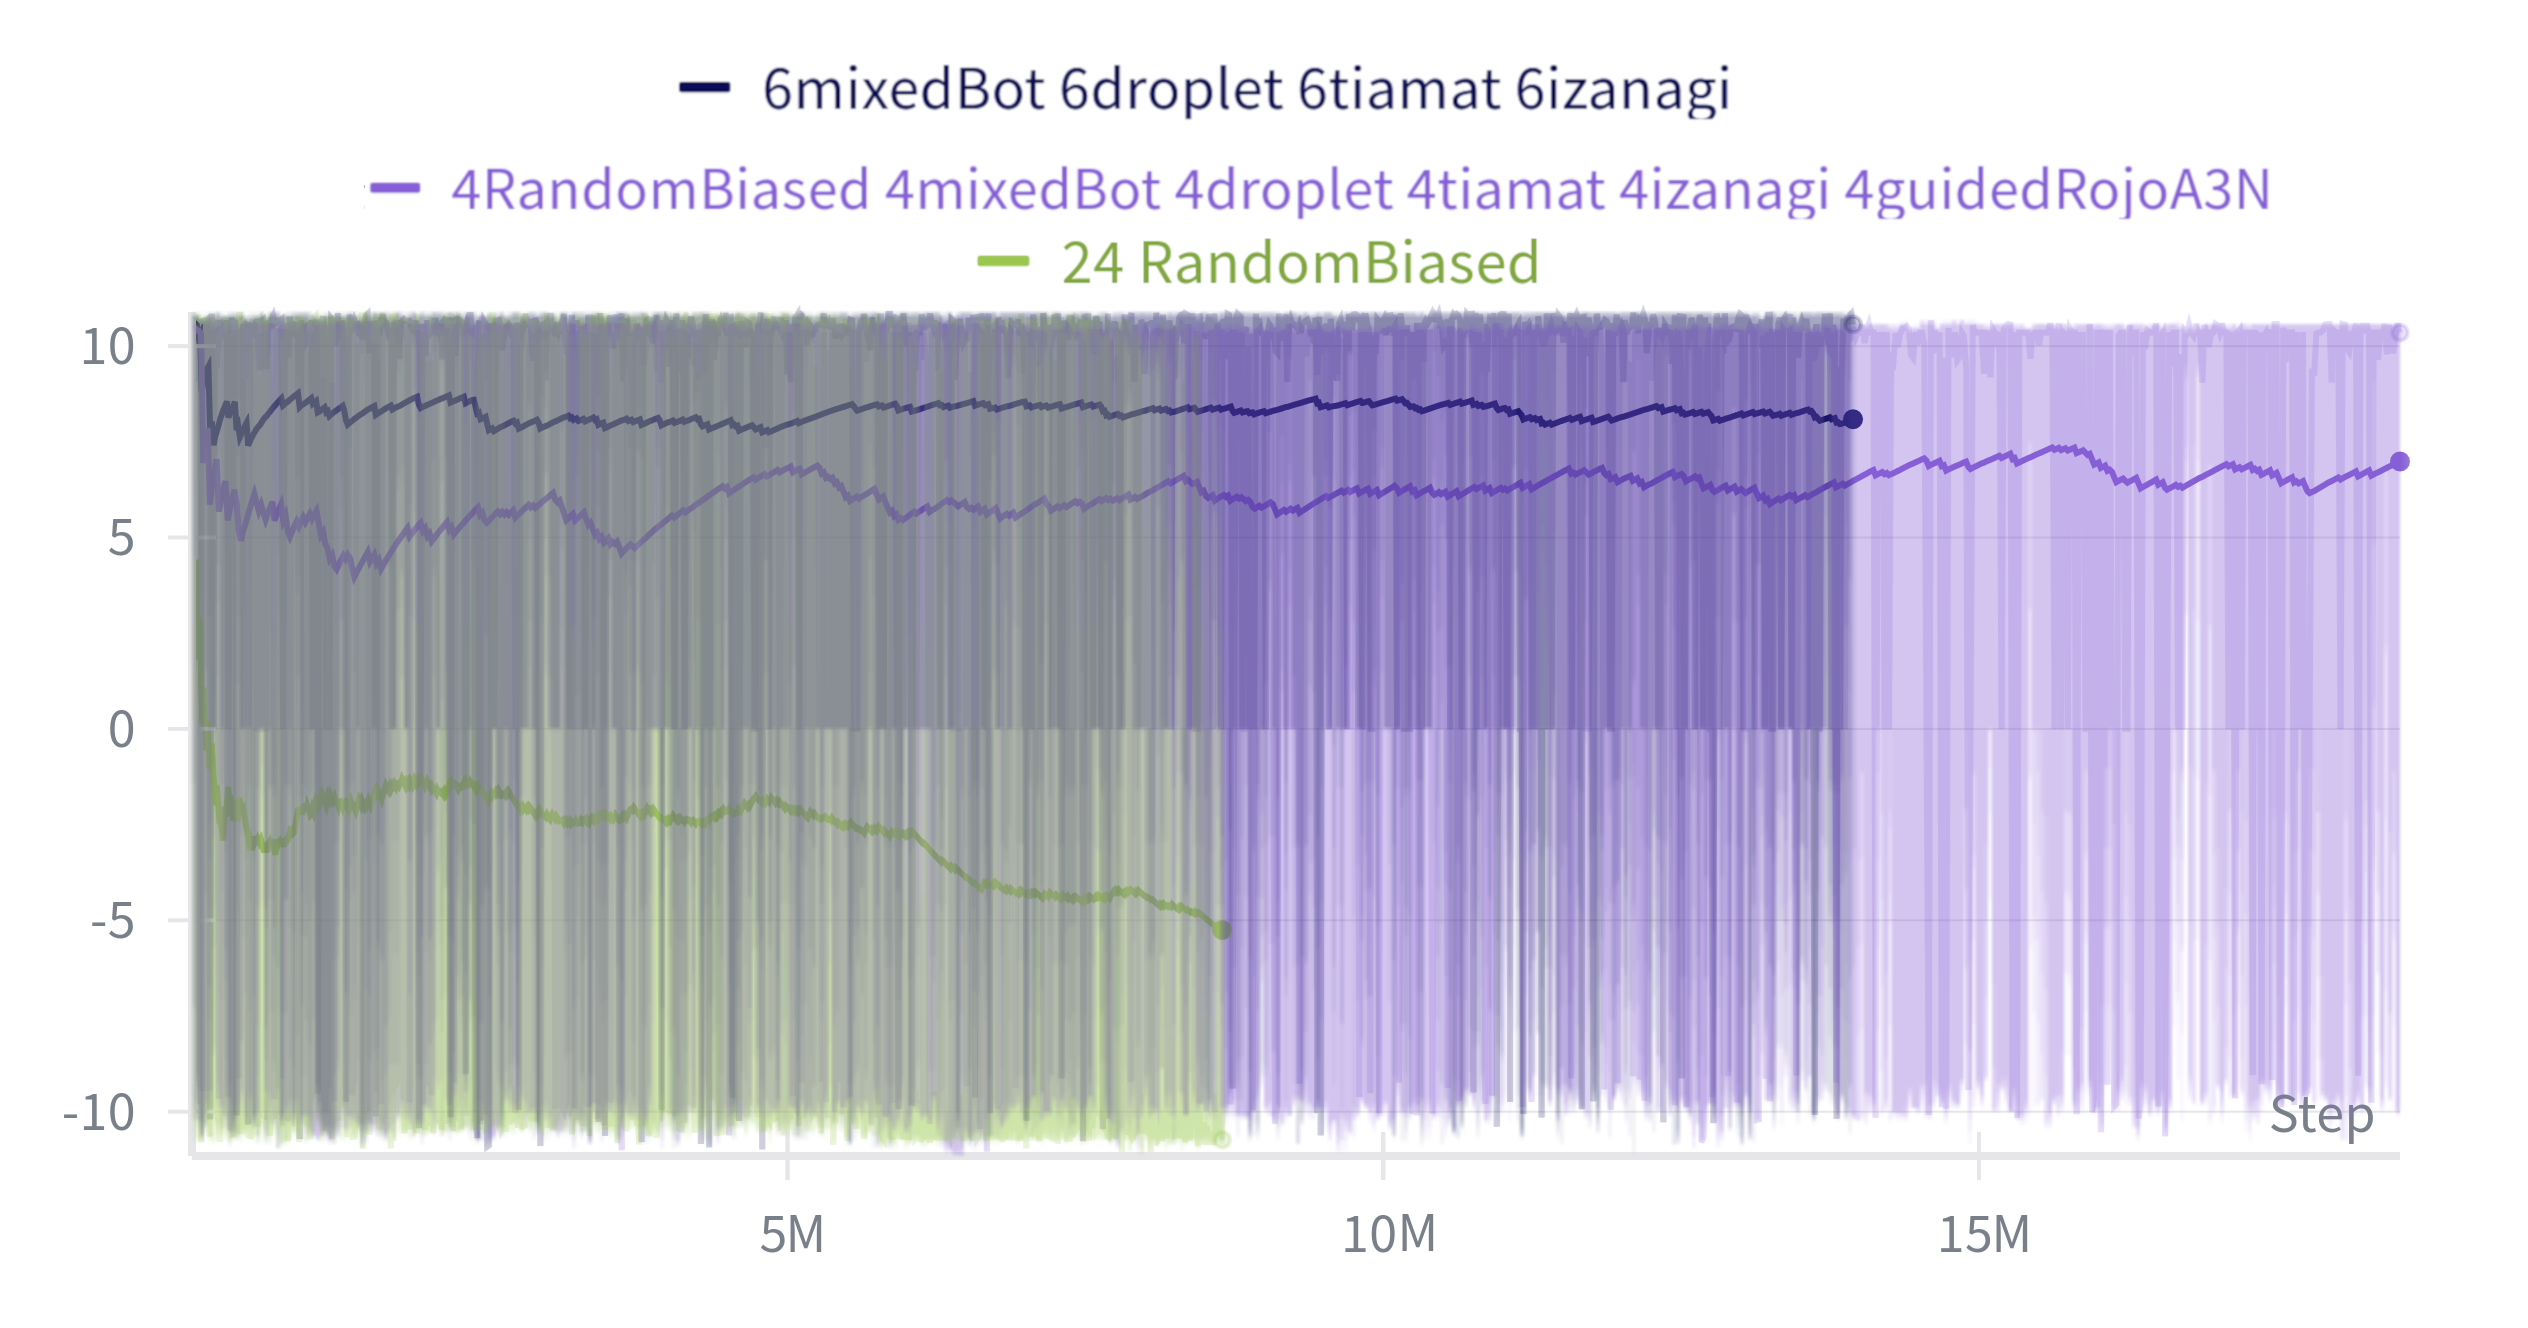
\includegraphics[width=1\linewidth]{images/Fig4.png}
    \caption{Episode rewards (y-axis) as a function of training timesteps (x-axis) on the final agent.}
    \label{Figure 4}
\end{figure}


% \subsection{Discussion}


\begin{itemize}
    \item \textbf{Generalization to random opponents:}
    \item \textbf{Map and observability constraints:} 
    \item \textbf{Replay and training bottlenecks:}
    \item \textbf{Exploitability:}
\end{itemize}


\section{Conclusion}
\label{sec:conclusion}



% \section{Reproducibility and Codebase}




%%%%%%%%% REFERENCES
{\small
\bibliographystyle{apalike}
\bibliography{references}
}

%%%%%%%%% Erkl\"arung
\onecolumn
\pagebreak\noindent
\textbf{\LARGE Erkl\"arung}
\addcontentsline{toc}{section}{Erkl\"arung}

\bigskip\bigskip
\noindent 
Hiermit versichere ich, dass ich die   Bachelorarbeit selbst\"andig verfasst und keine
anderen als die angegebenen Quellen und Hilfsmittel benutzt habe.

\bigskip
\noindent
D\"usseldorf, den XXXXXXXXXXX

\bigskip\bigskip\bigskip
\noindent
{Name!!!!!!!!!!!!!!!!!!!!!!!!!!!!!!!!!!!!!!!!!!!!!!!!!!!!!!!!!!!!!!!!!!!!!!!!!!!!!!}

\newpage

\end{document}
